\documentclass[12pt,twocolumn]{article}

\usepackage{fullpage}
\usepackage{listings}
\usepackage{graphicx}
\graphicspath{{images/}}
\usepackage{tabularx}
\usepackage{url}
\usepackage{hyperref}

\title{StreamReduce: Processing Data Streams\\and Avoiding Work}
\author{Ryan Lopopolo\\
Massachusetts Institute of Technology\\
\href{mailto:lopopolo@mit.edu}{\texttt{lopopolo@mit.edu}}}

\begin{document}
\maketitle

\section{Introduction}
\label{sec:intro}
One of the fundamental problems MapReduce was created to solve was processing
the growing amount of data in the world.
MapReduce lends itself naturally to top-k-style computations,
data sampling tasks, and other cases where perfect-fidelity results are not required.
Now with the open source Apache Hadoop
and Pig~\cite{Olston:2008:PLN:1376616.1376726}, it is easy to process and query
the terabytes of data an organization may collect.
%The widespread use of these tools to solve problems they weren't designed for motivates
%us to explore how we can save time, resources, and prevent faults in the execution of
%such MapReduce tasks.

With terabytes of data, however, it is scarcely necessary to examine
every entry to uncover trends, especially when one only cares about the most prominent
trends or results.
How does one decide which data to process then? Ultimately, this is problem dependent;
however, selctively deciding which data to
log is problematic because it can systemically mask some of the trends one would
try to uncover through analysis. In this paper, I introduce StreamReduce, a distributed system
for processing data streams. With StreamReduce I explore:
\begin{itemize}
  \item
    Randomly discarding data while trying to maintain a target accuracy level.
  \item
    Processing data using a variety of computation routines, some of which are less
    accurate than others.
\end{itemize}
Combining both of these techniques allows the cluster to save time by executing faster,
save resources by avoiding the need to process every datum, and minimize the impact of faults
in the execution of a job by treating failed tasks as discarded tasks.

Another limitation of MapReduce is batch processing. How does one
incorporate new data into an already analyzed task? MapReduce simply says to rerun
the job with the new data included. Others have solved this problem by batching data
into chunks and continuously spawning MapReduce jobs to incorporate the new data
and incrementally storing updates in an external database instead of relying on
the file system for enforcing the synchronization barrier.

A simpler way to incorporate new data is to treat data not as a constant, but as a
stream. By processing data on demand, one avoids repeating work involved in reprocessing
data, can save resources
by spinning workers up and down as necessary, and ensures results are as fresh as possible
by incorporating data into the result as soon as it arrives.

The goal of StreamReduce is to provide a MapReduce-style framework for processing streams. Such a
framework should include the ability to kill or discard tasks, be capable of
providing workers with serveral different computation routines to choose among, and pass data
between nodes using non-blocking routines.

\section{Related Work}
\label{sec:relwork}
% data stream management system
% continuous queries
%   sr doesn't do this, instead it operates on snapshots
%   this is how online mapreduce works
% append only data sets == Chronicle data model
%   views maintained incrementally without storing any chronicles (data items)
% sequencing of streams and sliding windows
%   sr doesn't do this
% Aurora - load shedding based on app specific QoS
% approximate answers
%   baked in to StreamReduce
%

StreamReduce builds of previous work in the areas of MapReduce, Data Stream Management Systems,
and approximation algorithms.

\subsection{MapReduce}
There is a rich research field around MapReduce. This section details work related to adapting
MapReduce to a streaming environment.

The Hadoop Online Prototype~\cite{Condie:EECS-2009-136} adds streaming to the MapReduce framework
by removing the materialize phase between mappers and reducers and between phases of a
MapReduce pipeline. Results are streamed from mappers to reducers as they become available.
At any given point, each reducer maintains an in-progress snapshot of the MapReduce job's
progress up to that point. This removes the synchronization barriers inherient in MapReduce
and allows incremental progress to be observed.

This approach is in contrast to the continuous query approach taken by many other streaming
systems. StreamReduce uses this snapshot approach.

\subsection{Data Stream Management Systems}
In their overview on data stream projects~\cite{Babcock:2002:MID:543613.543615},
a new class of data streaming applications
called \emph{Data Stream Management Systems} (\emph{DSMS}es) is discussed.
StreamReduce is a type of DSMS that includes some properties found in other systems.

The \emph{Chronicle Data Model}~\cite{Jagadish:1995:VMI:212433.220201} describes an
append-only stream of tuples. Such
streams lend themselves to incremental reads and incremental processing. In addition to incremental
updates, the Chronicle Data Model also seeks to update results incrementally without storing the
data itself.

The \emph{Data Stream Model}~\cite{Babcock:2002:MID:543613.543615} is a refinement of the Chronicle
Data Model. It has the following properties: stream items may arrive out of order,
streams are potentially unbounded in size, elements in the stream are discared after they are
processed. This is the data model that StreamReduce uses.

The Aurora system~\cite{Carney:2002:MSN:1287369.1287389} introduces the concept of
\emph{load shedding}, or compensating for
resource overload by comparing job specific quality of service metrics with target levels and
dropping items from the data stream.
StreamReduce aims to incorporate load shedding to dynamically tune jobs in the face of
impending time and resource constraints. On the other hand, it may be the case that
parts of a processing pipeline struggle to provide enough data to keep the next stage busy.
In this case, a streaming system would like to implement
\emph{early phase termination}~\cite{Rinard:2007:UEP:1297027.1297055}, or preemptively kill
a stage in the pipeline that is not capable of keeping all workers busy.

Aurora also introduces the non-blocking operators
\texttt{filter}, \texttt{map}, and \texttt{union} for
manipulating streams. StreamReduce implements these operators at the worker and fetcher nodes.

\subsection{Approximation Algorithms}
An alternative to load shedding to cope with high stream throughput is to perform approximate
computations on stream data.

Dynamic Knobs~\cite{Hoffmann:2011:DKR:1950365.1950390} describes a mechanism to explore the
accuracy-performance tradeoff space to adjust dynamically adjust program tuning parameters
to changes in the execution environment. This allows programs to do things such as
utilize more resources if they become available, use less power if power rates spike,
or use less accurate computations in the face of an impending time constraint.

The most important piece Dynamic Knobs offers to the DSMS space is dynamic
\emph{peak load provisioning}. Their system can adjust downward the amount of resources,
machines, etc. required for normal load and quickly adjust these levels back up to
handle load spikes. Combined with Aurora's load shedding, peak load provisioning can
be used to create a DSMS that uses less resources in both the normal and peak load
states.

Accuracy-aware transformations~\cite{Zhu:2012:RAP:2103656.2103710} are a class of transformations
that alter a computation according to a set of probabilstic weights and an accuracy
target such that the computation performs more efficiently. StreamReduce uses the subclass
of transformations called \emph{substitution transformations} in worker nodes to adjust
the runtime characteristics of per-datum computation.

The combination of load shedding, task killing and substitution transformations presents
an opportunity for the results of a computation performed by StreamReduce to be distorted.
Rinard~\cite{Rinard:2006:PAB:1183401.1183447} describes a method for bounding the distortion
introduced when discarding tasks. By breaking a computation into tasks, which in StreamReduce
consist of processing an individual datum at a worker, we can measure a
\emph{probabilistic distortion model} for a job, which gives bounds on its accuracy at different
task failure rates. I use this approach in the case study discussed in Section~\ref{sec:evaluation}.

\section{Design}
\label{sec:design}
StreamReduce is a distributed system for processing streams that can choose to kill tasks or
limit the amount of work it performs per task. Its design is modular and there are five
different types of nodes in a StreamReduce cluster:
\begin{itemize}
  \item
    \textbf{Spout}: A node external to the cluster that is a source of streaming data.
  \item
    \textbf{Fetcher}: Communicates with spouts to provide data for workers.
  \item
    \textbf{Worker}: Processes data returned by fetchers. They are the source of parallel computation
    in the cluster.
  \item
    \textbf{Collector}: Aggregates results from all workers and makes the result accessible via an API.
  \item
    \textbf{Master}: Manages the cluster by bringing nodes online to complete jobs. It is reponsible
    for all internode communication and storing to-be-processed data in several queues.
\end{itemize}
Figure~\ref{fig:systemdiagram} shows a system diagram of StreamReduce.

\begin{figure*}
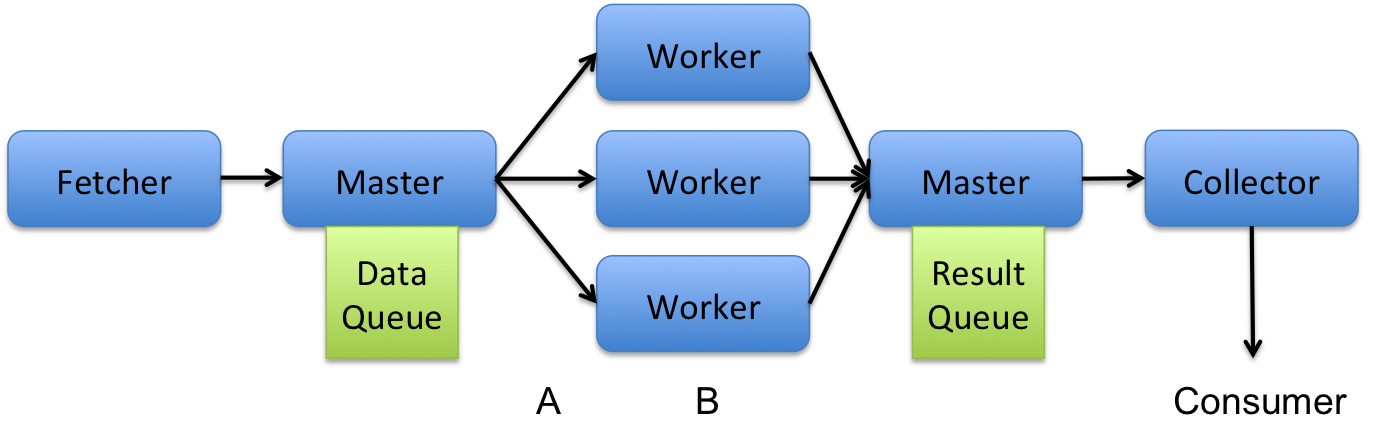
\includegraphics[width=\textwidth]{system-diagram.png}
\caption{Overview of data flow in the execution of a StreamReduce job. Load shedding occurs at point A. Task killing occurs at point B.}
\label{fig:systemdiagram}
\end{figure*}

\subsection{Spout}
Spouts are network-connected machines that generate data for a StreamReduce cluster to process.
Examples include a machine that tails a log file or an API like the Twitter tweet
stream. Fetchers depend on spouts as a source of streaming data.
\subsection{Fetcher}
Fetchers are responsible for communicating with spouts and returning data for the
workers to process. This level of indirection allows for a variety of different
configurations: A spout can emit data at such a high rate that using multiple fetchers
returns more data to the cluster, multiple fetchers can each talk to a different spout,
for example tailing logs from multiple machines, or fetchers can be set up redundantly
to ensure that every datum emitted by a spout is processed.

Fetchers may run indefinitely or return a status code indicating
the fetching task is over.
\subsection{Worker}
Workers perform processing on data provided by fetchers. They are similar to mappers
in the MapReduce framework. Each worker receives a fraction of the total input data
and each worker's tasks are independent of other workers'.

Workers are responsible for fulfilling the main design goals of StreamReduce. Workers may choose
to kill a task preemptively or, if it does not complete before a timeout, greedily. Additionally,
workers may choose among a variety of routines for performing computation on a datum.
Routines are ranked on a [0,1] scale based on the estimated fraction of total work it
requires. This rank is a proxy for the accuracy of a routine.

As it runs, a worker maintains an internal metric that estimates the fraction of work
it has performed over all data it has seen. Workers use this metric when choosing which
computation routine to run for a datum. A worker will choose the lowest ranked routine
such that its estimated fraction of work is above a configured threshold.
The total work estimator is used as a proxy for accuracy when a worker updates
this metric. This metric also takes into account the number of tasks it has killed
for any reason.

Because one of StreamReduce's goals is to process (potentially infinite) streams, workers do not
save their progress to disk and are forgetful; once the master queries a worker for its
progress and the worker successfully returns it, the worker clears all of its state and
continues processing. As a consequence, workers are easy to add or remove from the worker
pool because they don't need to be initialized with long-term job state. Additionally, as
long as the master polls workers frequently enough, only a small
fraction of the total work is lost upon worker failure.
The master queries workers every 100ms by default.
\subsection{Collector}
Collector nodes aggregate the results of all workers. Each collector acts as a reducer would
in the MapReduce framework if MapReduce used a single reducer for all of the mappers.
Collectors differ from MapReduce reducers in that they receive their data piecewise, as it
is produced from workers, as opposed to after all mappers have completed. This limits the
types of stateless aggregation collectors can do to online operations. (Of course, a collector
can choose to retain copies of individual worker results and re-reduce them each time more
results are receieved, but this is not in the spirit of the framework.)

Collectors also expose an API endpoint for accessing the results of a job. This endpoint
can be used by another spout to chain StreamReduce jobs together.
\subsection{Master}
\label{sec:master}
There is one master node per StreamReduce network. It has a function similar to the jobtracker in
MapReduce. New jobs are scheduled with the master and it initializes other nodes in the
cluster with job state. For each job, the master schedules roles among nodes in a round robin
manner to minimize the total number of outstanding roles on any one node.

The master is the only well-known node in the cluster. Other nodes in the network exclusively
communicate with the master. The master and other nodes communicate with each other by issuing
HTTP requests to a simple server on each node. I decided to make use of a library~\cite{sinatrarb}
providing the server functionality because there was a low barrier to getting inter-node
communication functioning. This design choice presents some problems and will be discussed
further in Section~\ref{sec:discussion}.

Another consequence of the master being the only well-known node is that all data in the
cluster must flow through it. The master maintains two queues per job for buffering job
progress from fetchers and workers and periodically pushes this state out to workers and
collectors, respectively.

\begin{figure}
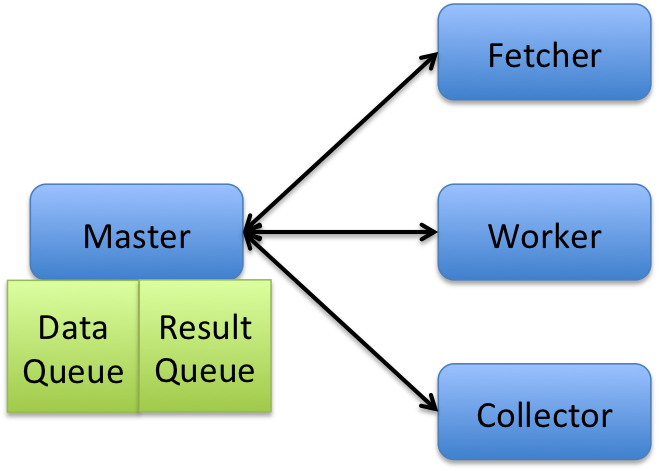
\includegraphics[width=\linewidth]{master-control-queue.png}
\caption{The master communicates directly with all nodes to pass them control messages. Nodes respond directly to the master with their results.}
\label{fig:mastercontrolqueue}
\end{figure}

Figure~\ref{fig:mastercontrolqueue} shows how control messages are passed from the master
to all other nodes in the cluster. The master communicates directly to each node and nodes
reply directly to the master when they have completed their task. With these control messages,
the master advances the state of the job. Such messages include telling a fetcher to fetch data
from a spout, giving data to a worker to process, and flushing results to collectors.


\subsection{Configuring a Cluster for a Job}
\label{sec:jobfile}
Apart from spouts, all nodes in a cluster modify their behavior based on the job they are
running. The master must know the appropriate number of nodes to spin up; fetchers need to
know how to talk to spouts; workers need to know how to compute results; and collectors need
to know how to combine batched worker results.

StreamReduce achieves this configuration with a Jobfile. Jobfiles are instances of a special class
provided by the StreamReduce framework. This class exposes several methods that can be invoked by a
given node to provide configuration parameters or execute code on its behalf. Most of the
routines that advance the progress of a StreamReduce job are wrappers around these Jobfile methods.

StreamReduce sends the source of the Jobfile to every node participating in the job and uses eval to
obtain a local instance of the Jobfile class. An example jobfile can be found at~\cite{github}.

The use of eval to instantiate Jobfile objects and the implementation language's (ruby)
ability to monkeypatch classes means that jobs can be modified on the fly just by sending
an updated Jobfile to job participants. For example, a job can be made lower fidelity in
the face of an impending time constraint, be made higher fidelity if more workers are added to
the cluster, or gracefully kill all fetchers which allows the job to end after all of the
various job queues are empty.
\subsection{Fault Tolerance}
StreamReduce can sustain the failure of any node other than the master. Because the master is responsible
for shuffling data between fetchers, workers, and collectors, a job cannot make progress without
the master.

Fetchers can fail. The only consequence of fetcher failure is that some of the input stream is
lost forever. Because StreamReduce uses the Data Stream Model, it does not attempt to recover this data.

Worker failures may entail some lost work. Having the master poll each worker frequently for its
progress mitigates the consequences of worker failure. For jobs that run for minutes or hours,
100ms of lost work is $\ll0.1\%$ of the total. StreamReduce can simply treat these lost tasks as preemptively
killed, which is already expected by the cluster.

Each collector is an exact replica of all others. Collector failure does not impact correctness of
the results delivered by any other collector. If no collectors are online, the data meant for them
sits in a queue on the master. Bringing another collector online will allow these and future results
to be aggregated.
\subsection{Killing Tasks and Working Less}
A design goal of StreamReduce is to compute meaningful results from a stream and to do so while not
processing every datum one-to-one. StreamReduce achieves this goal in two different ways. First, workers
may kill tasks preemptively to avoid the time and resource costs associated with processing
that task. Second, workers rely on the Jobfile to provide them with several different
computation routines of differing fidelities that perform a fraction of the total work on a
datum.

These behaviors appeal to the law of large numbers. It assumes that trends will still be
visible in spite of looking at only a fraction of the data. This means that the computation
routines and the weights assigned to them must be adapted to fit the distribution of the data
before the job starts (or updated \emph{in situ} via a new Jobfile).

\section{Methodology}
\label{sec:methodology}
The cluster I used to test StreamReduce is a 5-node network consisting of~1 spout,~1 fetcher,~4 workers,~1
collector, and~1 master. Roles were partitioned among nodes as shown in
Figure~\ref{fig:clusterDiagram}. Worker nodes were XVM~\cite{sipb:xvm} VMs provisioned with~128MB RAM each.
The master, spout, fetcher, and collector ran on a mid-2010 Macbook Air laptop with~4GB of RAM. I configured
the cluster to kill tasks on the master node, before they were shipped to workers.

\begin{figure}
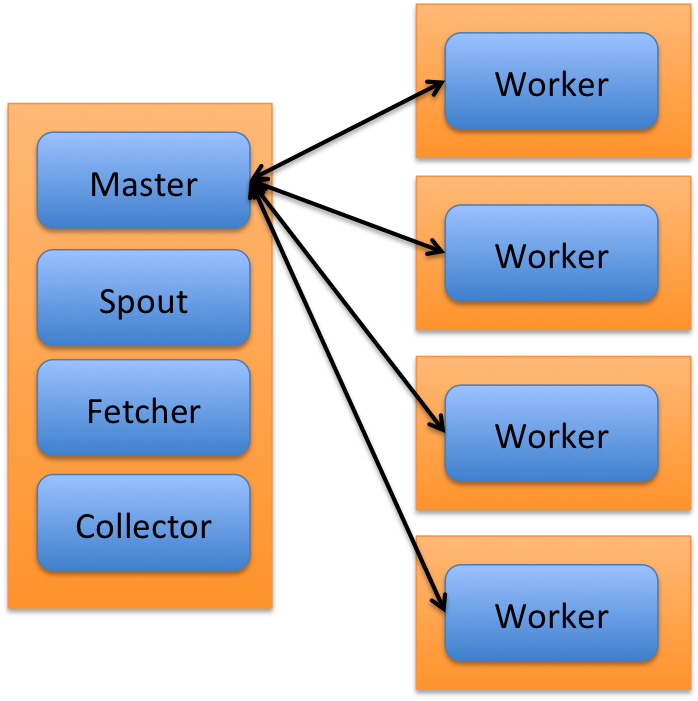
\includegraphics[width=\linewidth]{sr-topology.png}
\caption{Topology of the test StreamReduce cluster used in the word count case study. Each square box represents a single machine. Each rounded box represents a StreamReduce role.}
\label{fig:clusterDiagram}
\end{figure}

The job I ran was a word counter. The collector emits a hash whose keys are words and whose
values are the frequency the key occurred in the test corpus.

To run the job, I had to create a spout and find a source of data. For data, I acquired a
Wikipedia dump of the Featured Articles category. I used Wikipedia's xml
exporter~\cite{wikipedia:special:export} on January~9,~2012.

To serve the data, I transformed it into a YAML file containing a hash of
\begin{center}
$\texttt{article\_id}\rightarrow\texttt{fulltext}$.
\end{center}
To store fulltext, I base64 encoded it and
deflated it using zlib. This requires workers to inflate and decode the fulltext before they
can process it further. The server reads from this YAML file and returns the resulting hash as
JSON.

The fetcher communicates to the spout by requesting sequential article ids until it has fetched
every article.

Workers are initialized with the~3 computation routines shown in Table~\ref{table:workerTasks}.

\begin{table}
\begin{tabularx}{\linewidth}{|c|X|}
 \hline
Weight & Description \\ \hline
1.0 & Deflate and decode fulltext and count words in all of fulltext \\ \hline
0.25 & Deflate and decode fulltext and count words in approximately a quarter of fulltext \\ \hline
0.1 & Return the results of the last computation from a cache \\ \hline
\end{tabularx}
\caption{Computation routines used by StreamReduce workers.}
\label{table:workerTasks}
\end{table}

The results of the word count job were then used in a script to compute the top~100 words.
The cluster and word count job could be used in a two-stage top-k job. This script filters
out SEO stopwords~\cite{stopwords} to achieve more interesting results.

I ran four trials of the word count job for every combination of work level and task kill
rate I tested.

\section{Evaluation}
\label{sec:evaluation}
To evaluate StreamReduce, I explore the precision and recall of the word count test job as well as the
speedup factor associated with varying the task kill rate and target work level.

\subsection{Precision and Recall}
In order for task killing to be an effective strategy for a top-k computation, the
distribution of words in the corpus must be able to sustain data loss. This is the case
if the distribution is long-tailed, but is not true if the distribution is uniform.

\begin{figure}
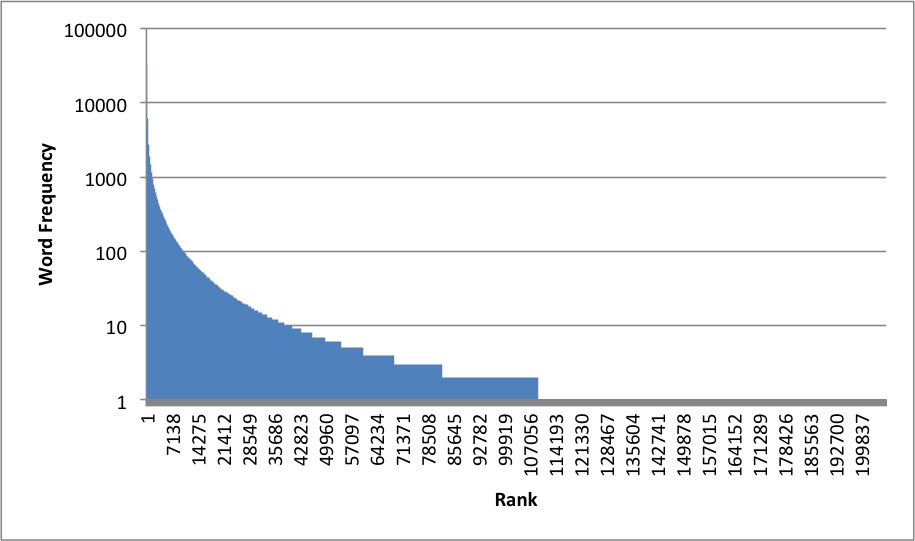
\includegraphics[width=\linewidth]{long-tail-ranks.png}
\caption{The frequencies of words in the Wikipedia Featured Articles corpus have a long-tailed distribution. This graph has had stopwords~\cite{stopwords} filtered out of it.}
\label{fig:wordDist}
\end{figure}

The distribution shown in Figure~\ref{fig:wordDist} is long-tailed. This implies that killing
tasks will impact the tail of the distribution more than the head.

\subsubsection{Precision}
Task killing should least impact the head of the word distribution.
Figure~\ref{fig:precision} shows that even with a task kill rate of~0.8 and a work level of~0.4,
meaning that the cluster only looks at 8\% of the words in the corpus, the results
are at least~80\% accurate. Increasing the work level, which increases the fidelity of
results emitted by workers, also increases the fidelity of the top~100 results.

\begin{figure}
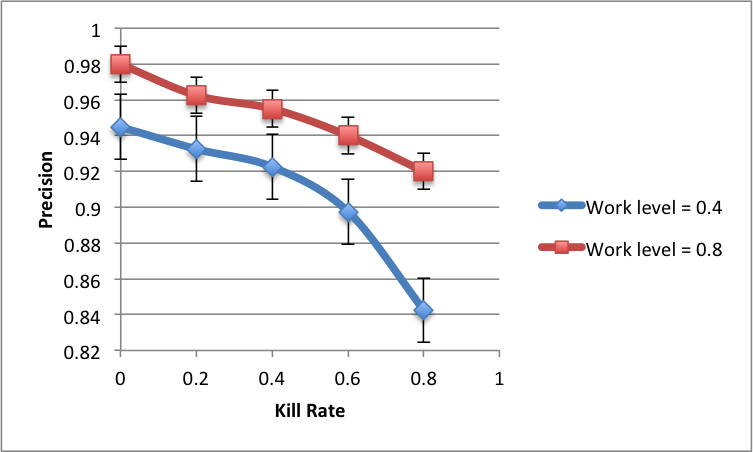
\includegraphics[width=\linewidth]{top-100-precision.png}
\caption{Fraction of the top~100 results returned in the top~100 by the word count job.}
\label{fig:precision}
\end{figure}

\subsubsection{Recall}
Recall in the tail of the distribution is most dependent on the work level of the word count job.
Anything less than perfect computation of a datum leaves out words with a frequency of one.
Figure~\ref{fig:recall} shows how recall improves as the work level increases. Task killing has
the same effect on recall as using low fidelity computation routines, so recall decreases as
the task kill rate does. Task killing dominates the impact of work level on recall as demonstrated
by the two lines converging in Figure~\ref{fig:recall}.

Poor recall statistics are acceptable because I am running a top-k job that focuses
on good precision in the top~100. Because I use a weighted $F$-score, the poor recall's impact
on measured accuracy is mitigated.

\begin{figure}
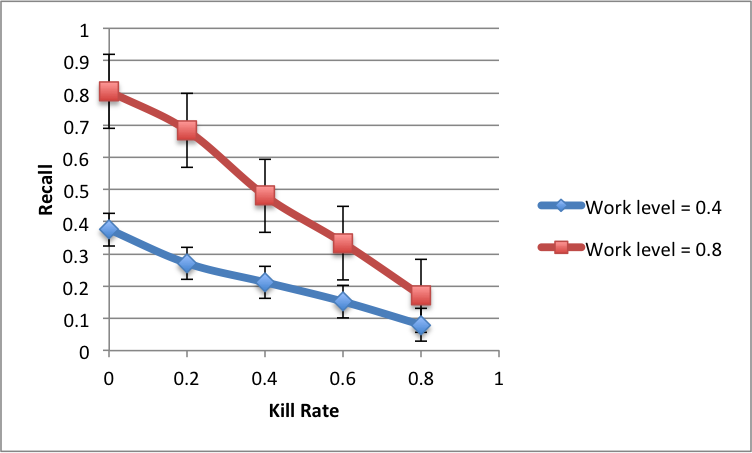
\includegraphics[width=\linewidth]{recall.png}
\caption{Fraction of the bottom~10000 results returned in the result set by the word count job.}
\label{fig:recall}
\end{figure}


\subsubsection{Word Count Job Accuracy}
Because I am running a top-k job, I compute the $F_{0.5}$-score of the StreamReduce results as
opposed to the $F1$-score because I care more about precision of the top k than recall
in the tail. Figure~\ref{fig:fscore} shows that the $F_{0.5}$-score, or the weighted
accuracy of the top-100 classifier, is always higher than the fraction of the input
examined (task kill rate * work level). Setting the work level to~0.4 nets a greater increase
in job accuracy versus fraction of words examined, with accuracy approximately~1.75 times
higher than the fraction of words examined.

\begin{figure}
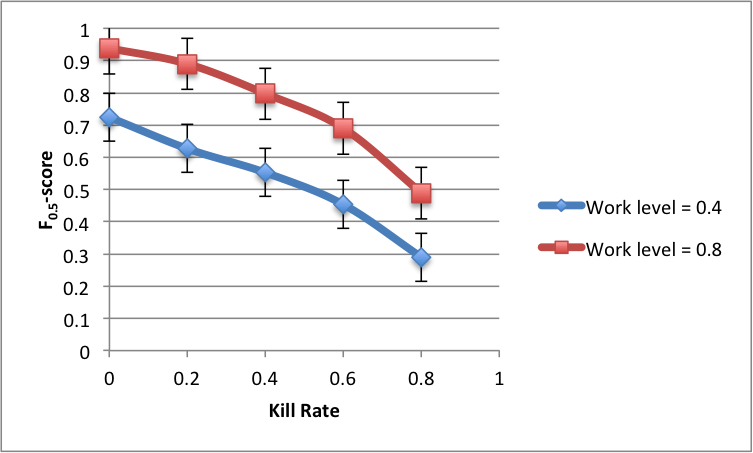
\includegraphics[width=\linewidth]{f-score.png}
\caption{$F_{0.5}$-score for the top-100 word count job. I measured the $F$-score with $\beta=0.5$ because the goal of the job is to run a top-k filter on it, meaning I care more about precision than recall.}
\label{fig:fscore}
\end{figure}

The average reduction in $F_{0.5}$-score caused by reducing the work level form 0.8 to 0.4 is
$0.231$ with a standard deviation of $0.025$. I performed four additional experiments with the
work level set to $0.8$ and $0.4$ with the task kill rate set to $0.1$ and $0.7$. These experiments were
not included in generating Figure~\ref{fig:fscore}. The average reduction in $F_{0.5}$-score between
work level $0.8$ and $0.4$ in these experiments is $0.230$ with a standard deviation of
$0.056$. These numbers show that a $0.4$ reduction in the work level leads to approximately a
$0.23$ reduction in $F_{0.5}$-score.

\subsection{Speedup}
StreamReduce is able to achieve a speedup over a MapReduce-style computation through three mechanisms:
providing multiple computation routines for the workers to choose from; varying the task kill
rate; and varying the target work level, which influences the chosen frequency of computation
routines per worker.

Table~\ref{table:runtime} shows the effect of varying the task kill rate and work level. The row
with kill~rate~$=0.0$ and work~level~$=1.0$ represents the perfect, MapReduce-style, execution
of the word count job. The only consistent reduction in execution time is a result of
increasing the task kill rate. Increasing the task kill rate exhibits a linear reduction in execution
time as the fraction of processed data linearly decreases.

\begin{table}
\begin{tabularx}{\linewidth}{|X|X|X|X|}
\hline
Task kill rate & Work level & Average execution time [s] & $F_{0.5}$-score \\ \hline\hline
0.0 & 1.0 & 696 & 1.000 \\ \hline
0.0 & 0.8 & 631 & 0.939 \\ \hline
0.0 & 0.4 & 634 & 0.725 \\ \hline\hline
0.2 & 1.0 & 531 & 0.933 \\ \hline
0.2 & 0.8 & 518 & 0.890 \\ \hline
0.2 & 0.4 & 506 & 0.627 \\ \hline\hline
0.4 & 1.0 & 393 & 0.829 \\ \hline
0.4 & 0.8 & 388 & 0.797 \\ \hline
0.4 & 0.4 & 414 & 0.552 \\ \hline\hline
0.6 & 1.0 & 292 & 0.774 \\ \hline
0.6 & 0.8 & 254 & 0.690 \\ \hline
0.6 & 0.4 & 255 & 0.453 \\ \hline\hline
0.8 & 1.0 & 144 & 0.541 \\ \hline
0.8 & 0.8 & 135 & 0.489 \\ \hline
0.8 & 0.4 & 153 & 0.290 \\ \hline
\end{tabularx}
\caption{Impact of task kill rate and work level on job execution time and $F_{0.5}$-score.}
\label{table:runtime}
\end{table}

Notably, simply by killing tasks, StreamReduce is able to achieve over a~5 times speedup compared
to the perfect execution while still returning about~84 of the top~100 words.

\subsection{Speed vs. Accuracy Tradeoffs}
\begin{center}
\begin{table*}
  \begin{tabularx}{\linewidth}{|lr|lr|lr|}
    \hline
    \multicolumn{2}{|X|}{Work level = 1.0 and task kill rate = 0.0} &
    \multicolumn{2}{|X|}{Work level = 0.8 and task kill rate = 0.4} &
    \multicolumn{2}{|X|}{Work level = 0.4 and task kill rate = 0.8} \\ \hline
    33225 & title & 21184 & title & 5982 & title \\ \hline
    29356 & web & 18398 & web & 4689 & web \\ \hline
    23095 & book & 13591 & journal & 4225 & journal \\ \hline
    21821 & journal & 13429 & book & 3629 & year \\ \hline
    20124 & year & 12770 & publisher & 3617 & publisher \\ \hline
    19786 & publisher & 12550 & url & 3444 & url \\ \hline
    19478 & url & 12220 & year & 3410 & book \\ \hline
    17360 & news & 11511 & news & 3273 & news \\ \hline
    16685 & accessdate & 11082 & united & 2968 & accessdate \\ \hline
    16401 & united & 10691 & accessdate & 2582 & world \\ \hline
  \end{tabularx}
  \caption{Example top~10 results and their frequencies from several different job configurations. The top~10 do not change much one changes the paramters to make the job less accurate.}
  \label{table:top10}
\end{table*}
\end{center}

Because the word distribution is so skewed toward the head, there is a great potential to
speed up the calculation by killing tasks without having to sacrifice too much accuracy.
Additionally, Table~\ref{table:runtime} shows that the most significant time savings comes
from increasing the kill rate and keeping the work level high yields about a~20 percentage point
increase in $F_{0.5}$-score.

The best combination of parameters is a high work level and as high a task kill rate one can
manage with respect to one's target distortion level.


\section{Implementation Notes}
\label{sec:discussion}
This section describes deficiencies in the implementation of StreamReduce used to run the case study
in this paper and goals for the next version of the system.

\subsection{On-the-Fly Job Reconfiguration}
The mechanism for altering execution of a job as it is running described in Section~\ref{sec:jobfile}
is not yet implemented. Adding this feature to StreamReduce is a matter of adding an API endpoint
to the servers run by each role and adding a bin-script to submit the new Jobfile.

\subsection{Internode Communication}
In Section~\ref{sec:master} I mentioned design difficulties relating to the master and using HTTP
requests for sending messages between nodes. I initially chose to use HTTP requests with POST payloads
to send data and results between nodes because of its low barrier to entry; however, initiating many
HTTP requests in succession is expensive. When killing jobs on worker nodes, the observed time savings
was minimal because most of the time spent per datum involved shipping it from the master to the worker.

In order to mitigate the effects of this problem, I batched individual requests into groups of~5. This
lowered the number of connections I was initiating but it also limited the parallelism of the cluster
and removed workers from the pool for longer periods because they had more data to process at a time.
A killed task on the worker no longer freed it up to receive a new task immediately.
Keeping workers removed from the pool caused the queues on the master to grow longer as the workers
could no longer keep up with the rate the fetcher was producing data.

Eventually, I introduced a configuration option to kill tasks at the master. The master then
decides to discard a task as it is popped from the queue, before it is ever sent to a worker.
Doing so improved the execution time of the cluster but also meant that workers no longer had
a full idea of how accurate they were being because they never killed any tasks themselves.

In order to address this problem, the master needs to keep a persistent channel open between
it and all active nodes. Communication channels should be established when nodes come online.
Possible solutions include writing to a socket or using a higher abstraction like AMPQ\@.
AMPQ is appealing because it also relieves the master from handling queues.

\subsection{Node Health}
Currently, the master does not probe nodes to ensure that they are responsive. In the case that
a node is serving a worker role for a job, this deficiency is masked. The node will simply not
return the HTTP request sent to it to push it some data and the worker will remain removed from
the pool. If the node is in the role of fetcher or collector, the master will stall.

All messages passed by the master to other nodes must be made non-blocking.

\subsection{Job Management}
There is no support for killing jobs or removing them from the master's data structures. The only
way to remove a job is to kill the master and all other nodes in the cluster.

\section{Conclusion}
I have extended the ideas of approximate computations to a MapReduce-style framework and shown
that it is feasible to tune the input parameters of a job to achieve sufficient precision and
recall for a particular application.

I have taken a different approach to streaming MapReduce by treating data not as a batch, but
as a stream. At any given point in the execution of a job, the collectors will have accurate
(so far as the job parameters allow) results for data seen until that point. This approach
guarantees freshness and makes it easier to incorporate new data into an existing computation,
yet it suffers from being limited to online aggregations.

The StreamReduce source code is open source and available at:
\begin{center}
  \url{https://github.com/lopopolo/sr}
\end{center}

\subsection*{Acknowledgments}
I would like to acknowledge Martin Rinard for giving me direction for my initial idea
and guiding me to apply the data stream model to StreamReduce; Sasa Misailovic for being
a sounding board for ideas and providing me with background research; Daniel Erenrich for
providing information about data stream management systems; and SIPB for providing the
XVM service, which made deploying a StreamReduce cluster painless.

\bibliography{paper}{}
\bibliographystyle{plain}

\end{document}
